%\documentclass[13pt,aspectratio=169]{beamer}% Used to establish the beamer environment
%
\documentclass[20pt]{beamer} % scale up the font largest available is 20
\geometry{papersize={16in,9in}} % make much larger. needs testing
%
%
\usepackage{tikz} % Used for vectorized drawings
\usetikzlibrary{shapes.geometric}
\usetikzlibrary{math}
%
\usepackage{amsmath} % Math typesetting package
\usepackage{amssymb} % Math symbols
\usepackage{float}  % Defines floating objects (Tables, Figures, etc...)
%\usepackage{pgfplots} % Package for plotting


\usepackage{color,soul} % 
\usepackage{mathtools}
\usepackage{appendix}
\usepackage{siunitx}
\usepackage[normalem]{ulem}
\usepackage{upgreek}
\usepackage[numbers]{natbib}
\usepackage{subfigure}
\usepackage{miller}
% Theme choice (black and white, essentially)
\usecolortheme{dove}

% Frame titles
\setbeamerfont{frametitle}{size=\Large,series=\bfseries}
% Block title settings
\setbeamerfont{block title}{size=\large,series=\bfseries}

% Footer with acme lab, logo and frame number 
\addtobeamertemplate{footline}{%
  \begin{tikzpicture}
    % Crimson PMS 201
    \definecolor{mycolor}{RGB}{158,27,50}
    %
    \filldraw[color=mycolor, fill=mycolor, very thick] (-2,-1) rectangle (\textwidth,.27);
    
    \node[right, anchor= south west, text =white] (logo) at  (-2,-1) {
\includegraphics[width= 1cm]{figures/A-Square-Logo-4c_Official.jpg}};
    
    \node[right, anchor=west, text =white] at (logo.east) {\normalsize ACME Lab};
    
   \node [left,anchor=south east, text =white] at (.93\textwidth,-.67) {\normalsize \insertframenumber{}};
\end{tikzpicture}}

% Removes navigation symbols
\setbeamertemplate{navigation symbols}{}

% Title and author
\title{Slip system anisotropy study}
\author{Ezra Mengiste, Matthew Kasemer}
\setbeamerfont{title}{size=\Huge}

%%%%% Begin document
\begin{document}

% Make title page
\maketitle
% Include body slides here
%\begin{frame}{Simulation test matrix}
    \begin{table}[]
    \scriptsize
        \centering
        \begin{tabular}{|c|c|c|c|c|c|c|c|c|c|c|c|c|}
        \hline
            Simulation &$\hkl(0 1 -1)$ $\hkl[1 1 1]$   &$\hkl(1 0 -1)$ $\hkl[1 1 1]$   &$\hkl(1 -1 0)$ $\hkl[1 1 1]$   &$\hkl(0 1 1)$  $\hkl[1 1 -1]$  &$\hkl(1 0 1)$  $\hkl[1 1 -1]$  &$\hkl(1 -1 0)$ $\hkl[1 1 -1]$  &$\hkl(0 1 1)$  $\hkl[1 -1 1]$  & $\hkl(1 0 -1)$ $\hkl[1 -1 1]$  &$\hkl(1 1 0)$  $\hkl[1 -1 1]$  &$\hkl(0 1 -1)$ $\hkl[1 -1 -1]$ &$\hkl(1 0 1)$  $\hkl[1 -1 -1]$ &$\hkl(1 0 1)$  $\hkl[1 -1 -1]$ \\ \hline \hline
            %\hline
            %&0&1&2&3&4&5&6&7&8&9&10&11\\
             Control    & 39.0    & 39.0    & 39.0    & 39.0& 39.0   & 39.0     & 39.0    & 39.     0& 39.0     & 39.0   & 39.0    & 39.0    \\ \hline \hline  
             First Set  & 39.0    & 39.0    & 39.0    & 39.0& 39.0    & 39.0    & $\infty$& $\infty$&  $\infty$& $\infty$& $\infty$& $\infty$\\ \hline
             Second Set & 39.0    & $\infty$& $\infty$& 39.0& $\infty$& $\infty$& 39.0    & $\infty$& 39.0     & 39.0    & $\infty$& 39.0    \\ \hline
             Third Set (new 2) & $\infty$& $\infty$& 39.0    & 39.0& 39.0    & $\infty$& 39.0    & $\infty$& 39.0     & $\infty$& 39.0    & $\infty$\\ \hline 
             \hline
             
        \end{tabular}
    \end{table}
\end{frame}
%\begin{frame}
    %
    \frametitle{Example Figure}
    %
    Here is an example of a figure, which you can reference as Figure~\ref{fig:label}:
    \begin{figure}
        \centering
        \includegraphics[width=0.5in]{figures/miller_indices.png}
        \caption{This is a caption for the figure}
        \label{fig:my_label}
    \end{figure}
    %
    You can also have sub-figures, which can make having multiple plots on a slide easy:
    \begin{figure}
        \centering
        \subfigure[]{
            \includegraphics[width=0.5in]{figures/miller_indices.png}
        }
        \quad
        \subfigure[]{
            \includegraphics[width=0.5in]{figures/miller_indices.png}
        }
        \caption{This is an example subfigure.}
        \label{fig:my_label2}
    \end{figure}
    %
\end{frame}
\newcommand{\study}[1]{
\newif\ifhiggs

\IfFileExists{abc.tex}{\higgstrue}{\higgsfalse}
\ifhiggs
  \loop
  \begin{frame}
  \repeat
\fi
}
% if 
\newcommand{\widP}{2.4in}
\newcommand{\widF}{2.4in}
\newcommand{\simu}{one}
% RUN NEW CONTROL SIMS
\newcommand{\polycube}{\includegraphics[width=\widP]{figures/cubic_domain_control_density.png}}
\newcommand{\polyelongated}{\includegraphics[width=\widP]{figures/elongated_domain_control_density.png}}
%
\newcommand{\cTimesOTF}[2]{\includegraphics[width=\widF]{figures/Cube_125_#1ss_set_#2_density.png}}
\newcommand{\cTimesOFO}[2]{\includegraphics[width=\widF]{figures/Cube_150_#1ss_set_#2_density.png}}
\newcommand{\cTimesOSF}[2]{\includegraphics[width=\widF]{figures/Cube_175_#1ss_set_#2_density.png}}
\newcommand{\cTimesTH }[2]{\includegraphics[width=\widF]{figures/Cube_200_#1ss_set_#2_density.png}}
\newcommand{\cTimesFH }[2]{\includegraphics[width=\widF]{figures/Cube_400_#1ss_set_#2_density.png}}
%
\newcommand{\eTimesOTF}[2]{\includegraphics[width=\widF]{figures/Elongated_125_#1ss_set_#2_density.png}}
\newcommand{\eTimesOFO}[2]{\includegraphics[width=\widF]{figures/Elongated_150_#1ss_set_#2_density.png}}
\newcommand{\eTimesOSF}[2]{\includegraphics[width=\widF]{figures/Elongated_175_#1ss_set_#2_density.png}}
\newcommand{\eTimesTH }[2]{\includegraphics[width=\widF]{figures/Elongated_200_#1ss_set_#2_density.png}}
\newcommand{\eTimesFH }[2]{\includegraphics[width=\widF]{figures/Elongated_400_#1ss_set_#2_density.png}}
%
\newcommand{\tablee}[1]{ 
\footnotesize{
    \begin{tabular}{|c|c|c|c|c|c|c|c|c|c|c|c|c|}
        \hline
        Simulation &$\hkl(0 1 -1)$ $\hkl[1 1 1]$   &$\hkl(1 0 -1)$ $\hkl[1 1 1]$   &$\hkl(1 -1 0)$ $\hkl[1 1 1]$   &$\hkl(0 1 1)$  $\hkl[1 1 -1]$  &$\hkl(1 0 1)$  $\hkl[1 1 -1]$  &$\hkl(1 -1 0)$ $\hkl[1 1 -1]$  &$\hkl(0 1 1)$  $\hkl[1 -1 1]$  & $\hkl(1 0 -1)$ $\hkl[1 -1 1]$  &$\hkl(1 1 0)$  $\hkl[1 -1 1]$  &$\hkl(0 1 -1)$ $\hkl[1 -1 -1]$ &$\hkl(1 0 1)$  $\hkl[1 -1 -1]$ &$\hkl(1 0 1)$  $\hkl[1 -1 -1]$ \\ \hline \hline
        %\hline
        %&0&1&2&3&4&5&6&7&8&9&10&11\\
         Strength #    & 39.0    & 39.0    & 39.0    & 39.0& 39.0   & 39.0     & 39.0    & 39.     0& 39.0     & 39.0   & 39.0    & 39.0    \\ \hline             
    \end{tabular}}
}
%
\newcommand{\simulation}[3]{
\begin{frame}{Simset number #3: #1 slip systems altered set #2}
    \begin{table}[]
        \centering
        \begin{tabular}{|c|ccccc|} 
        \hline
        Isotropic & 125\% & 150\% & 175\% & 200\% & 400\% &
        \hline
             \polycube&      \cTimesOTF{#1}{#2}& \cTimesOFO{#1}{#2}& \cTimesOSF{#1}{#2}& \cTimesTH{#1}{#2}& \cTimesFH{#1}{#2} \\
             \hline
             \polyelongated& \eTimesOTF{#1}{#2}& \eTimesOFO{#1}{#2}& \eTimesOSF{#1}{#2}& \eTimesTH{#1}{#2}& \eTimesFH{#1}{#2}\\
            \hline
        \end{tabular}
    \end{table}
    %\tablee{#3}
\end{frame}
}
\simulation{2}{1}{001-005}
\simulation{2}{2}{006-010}
\simulation{2}{3}{011-015}
\simulation{2}{4}{016-020}
\simulation{2}{5}{021-025}

\simulation{4}{1}{026-030}
\simulation{4}{2}{031-035}
\simulation{4}{3}{036-040}
\simulation{4}{4}{041-045}
\simulation{4}{5}{046-050}

\simulation{6}{1}{051-055}
\simulation{6}{2}{056-060}
\simulation{6}{3}{061-065}
\simulation{6}{4}{066-070}
\simulation{6}{5}{071-075}
%\newcommand{\study}[1]{
\newif\ifhiggs

\IfFileExists{abc.tex}{\higgstrue}{\higgsfalse}
\ifhiggs
  \loop
  \begin{frame}
  \repeat
\fi
}
% if 
\newcommand{\widP}{1.5in}
\newcommand{\widF}{2.5in}
\newcommand{\simu}{one}
%
\newcommand{\polycube}{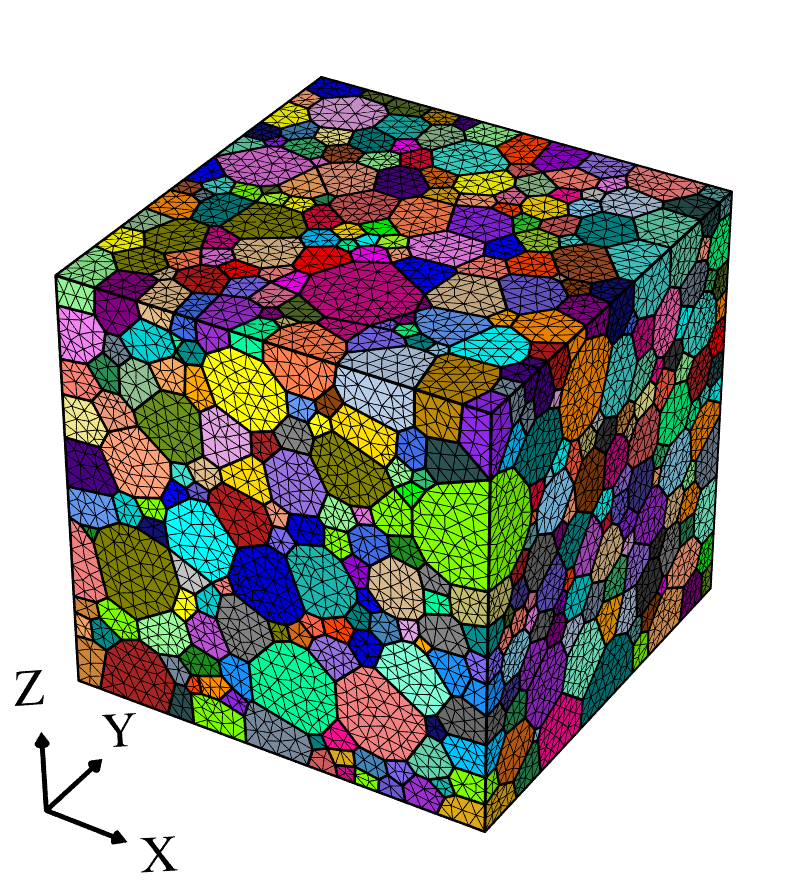
\includegraphics[width=\widP]{figures/cubic_domain.png}}
\newcommand{\polyelongated}{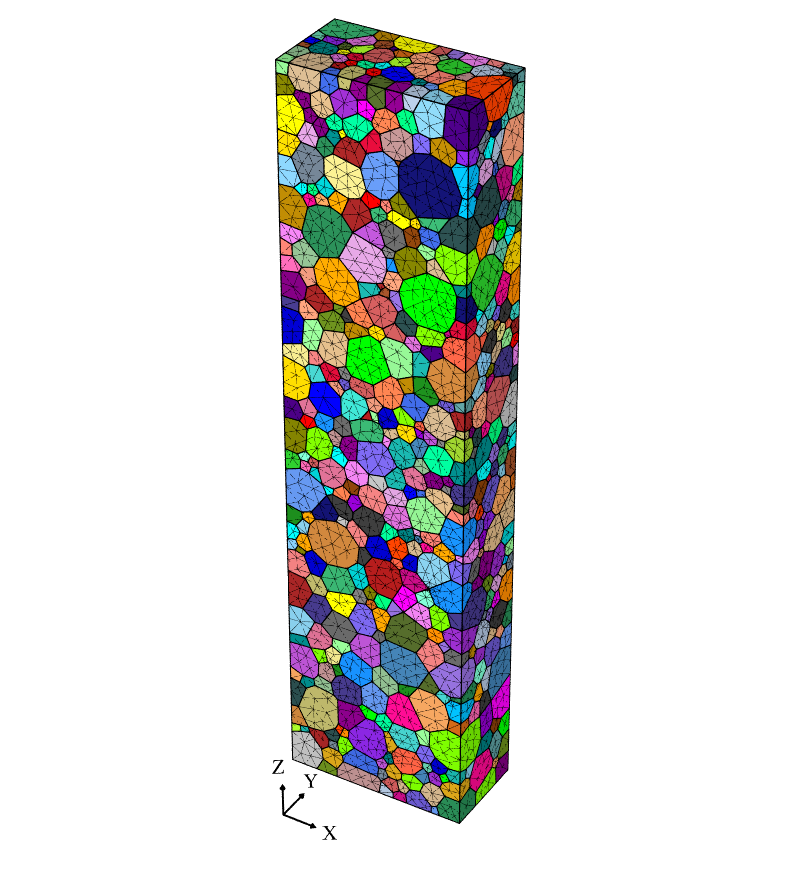
\includegraphics[width=\widP]{figures/elongated_domain.png}}
%
\newcommand{\cTimesOTF}[2]{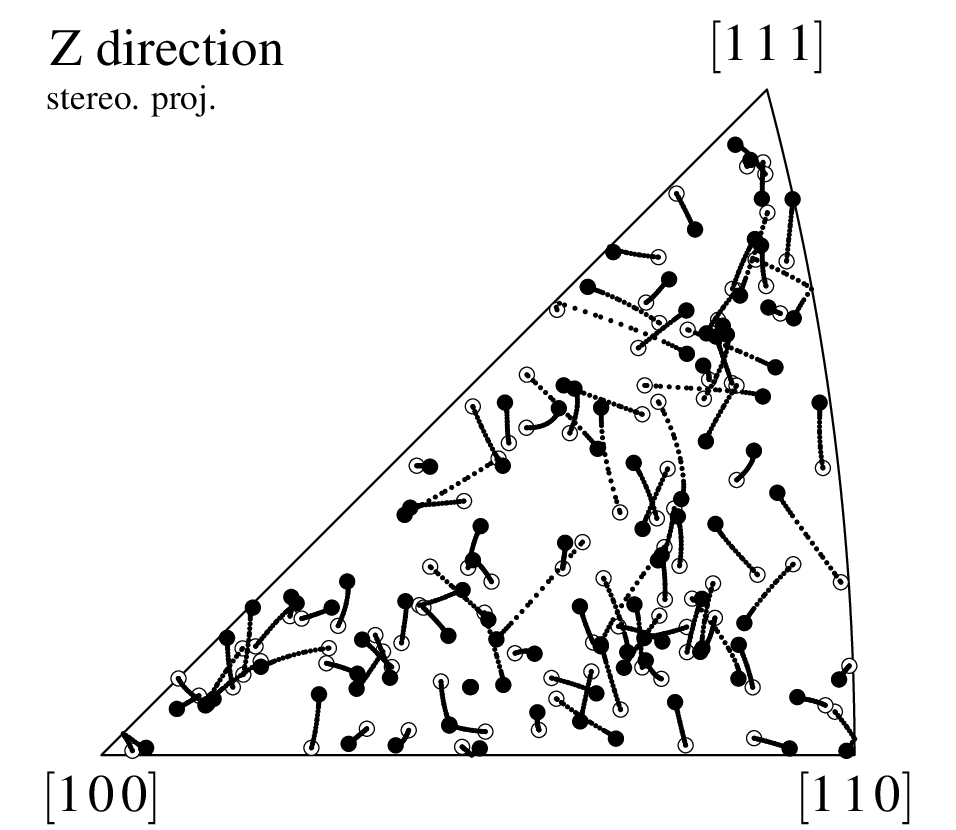
\includegraphics[width=\widF]{figures/testing_fig.png}}
\newcommand{\cTimesOFO}[2]{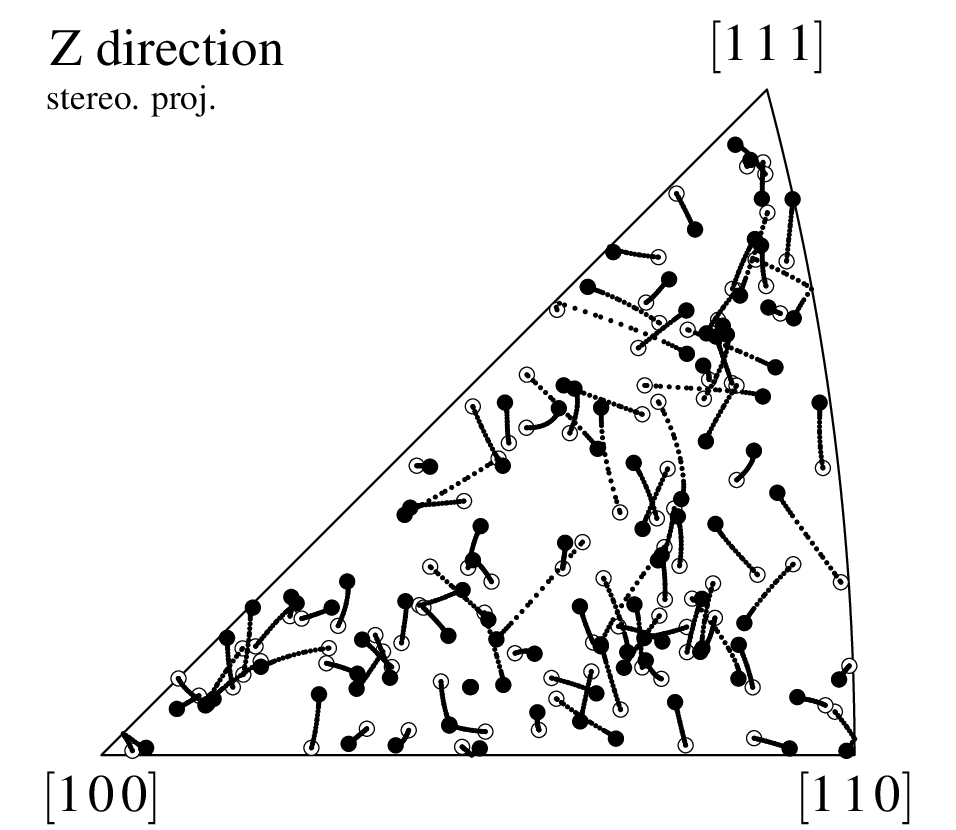
\includegraphics[width=\widF]{figures/testing_fig.png}}
\newcommand{\cTimesOSF}[2]{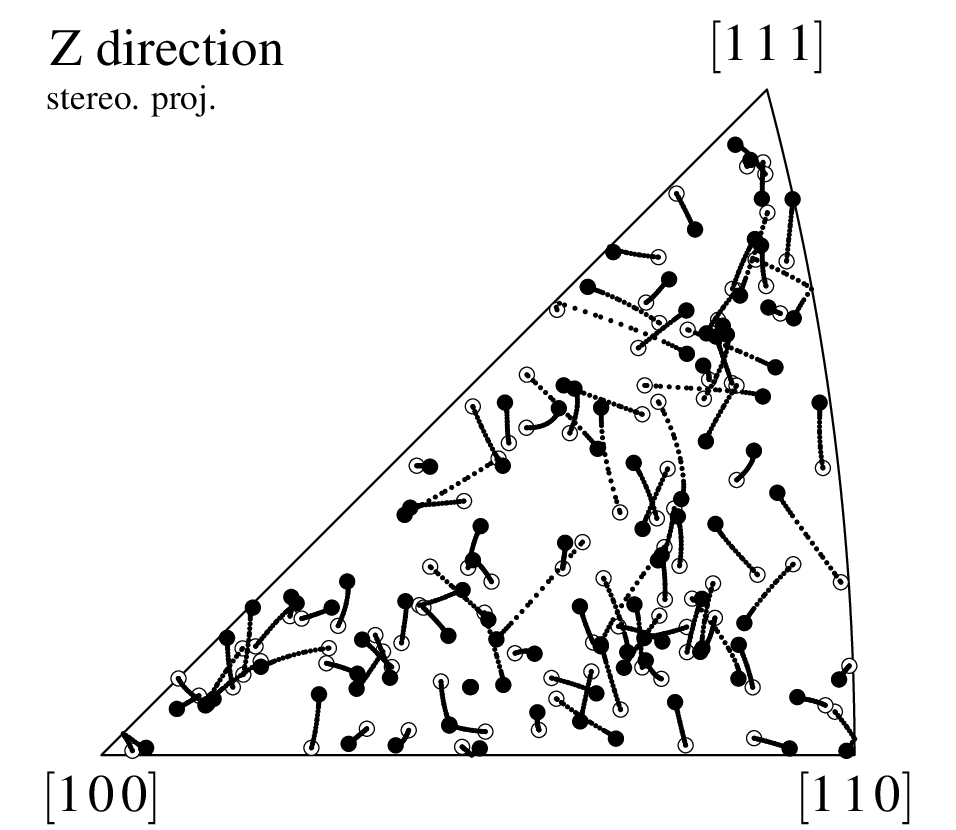
\includegraphics[width=\widF]{figures/testing_fig.png}}
\newcommand{\cTimesTH }[2]{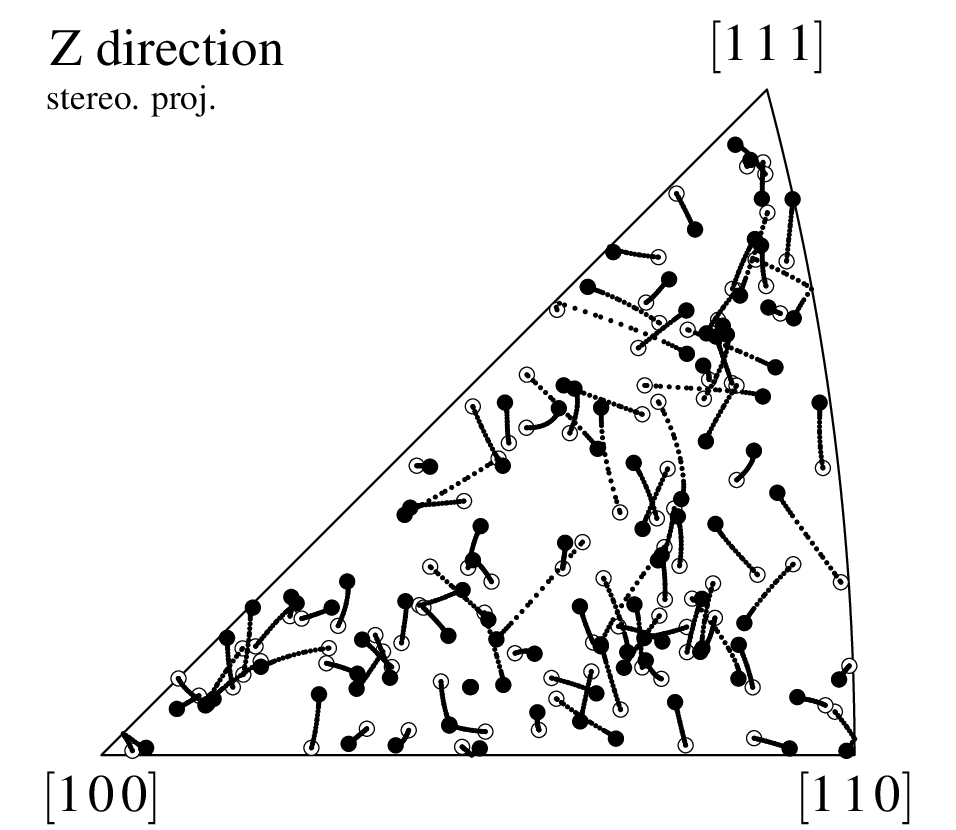
\includegraphics[width=\widF]{figures/testing_fig.png}}
\newcommand{\cTimesFH }[2]{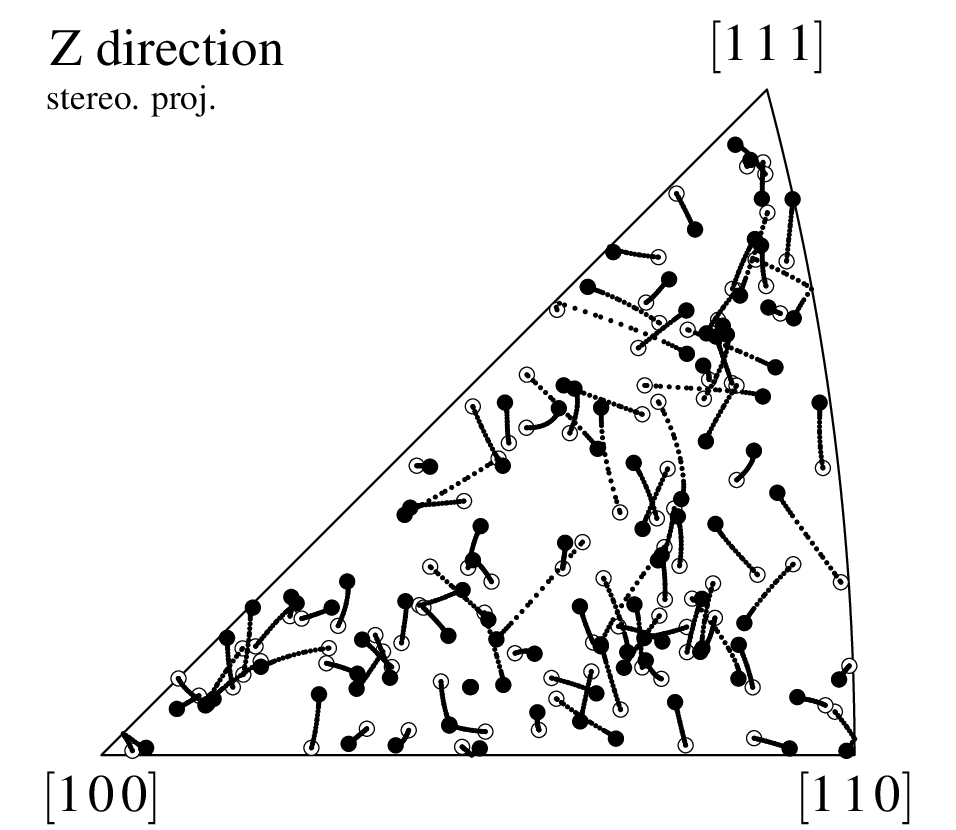
\includegraphics[width=\widF]{figures/testing_fig.png}}
%
\newcommand{\eTimesOTF}[2]{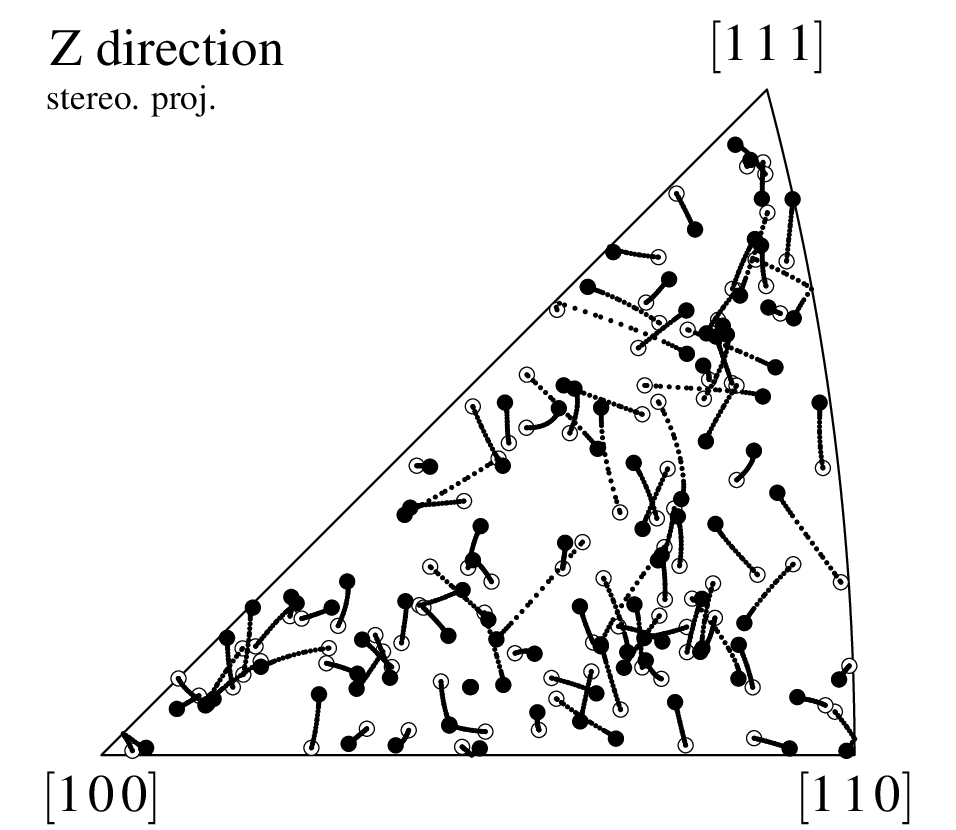
\includegraphics[width=\widF]{figures/testing_fig.png}}
\newcommand{\eTimesOFO}[2]{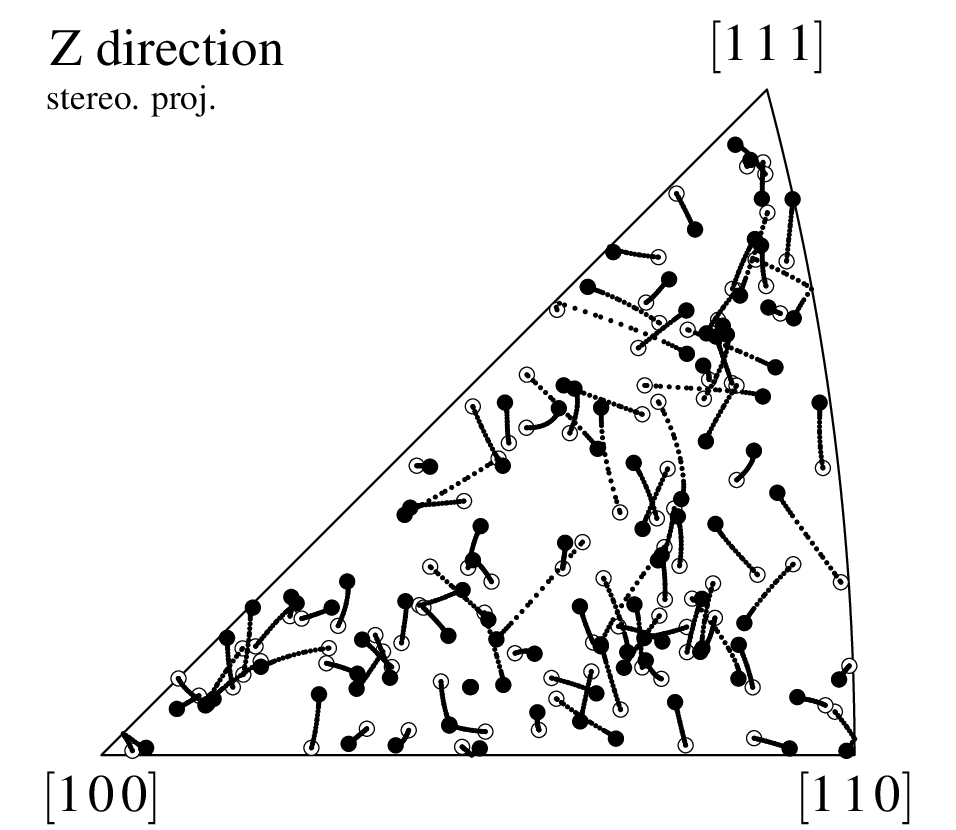
\includegraphics[width=\widF]{figures/testing_fig.png}}
\newcommand{\eTimesOSF}[2]{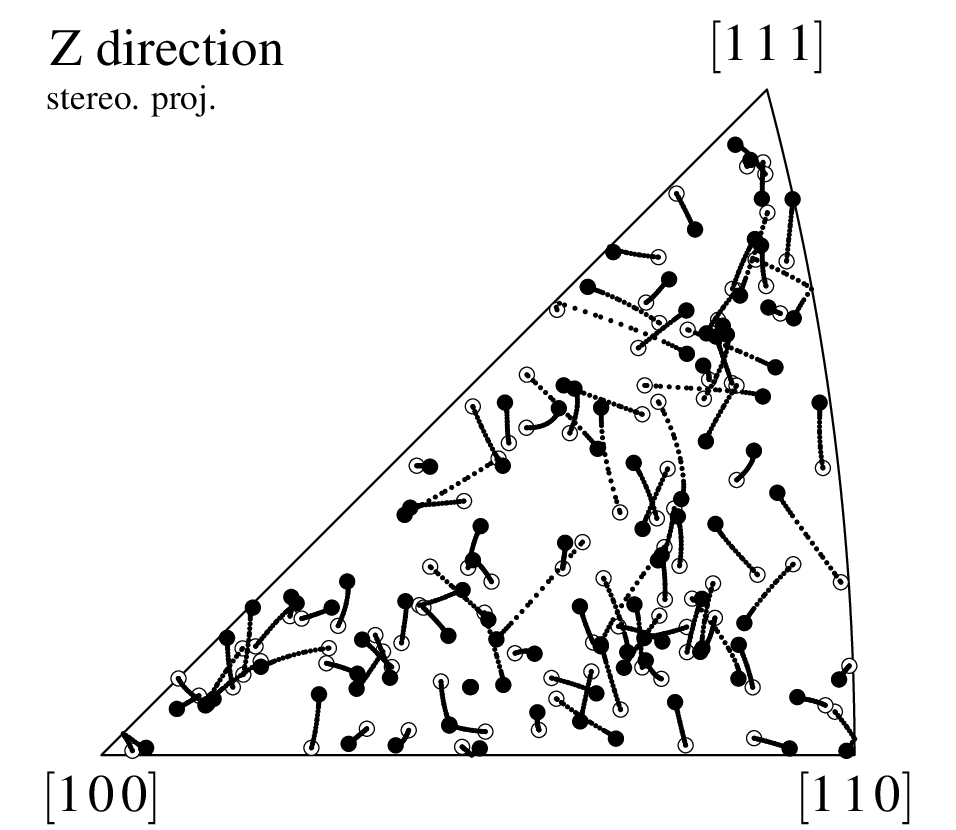
\includegraphics[width=\widF]{figures/testing_fig.png}}
\newcommand{\eTimesTH }[2]{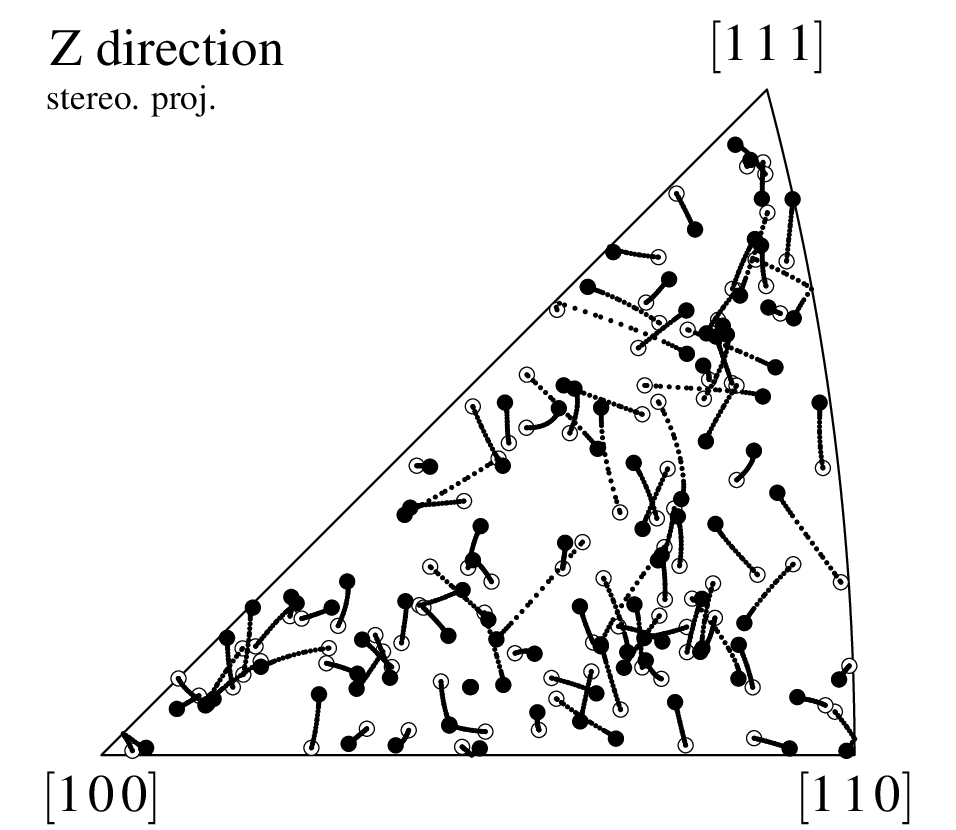
\includegraphics[width=\widF]{figures/testing_fig.png}}
\newcommand{\eTimesFH }[2]{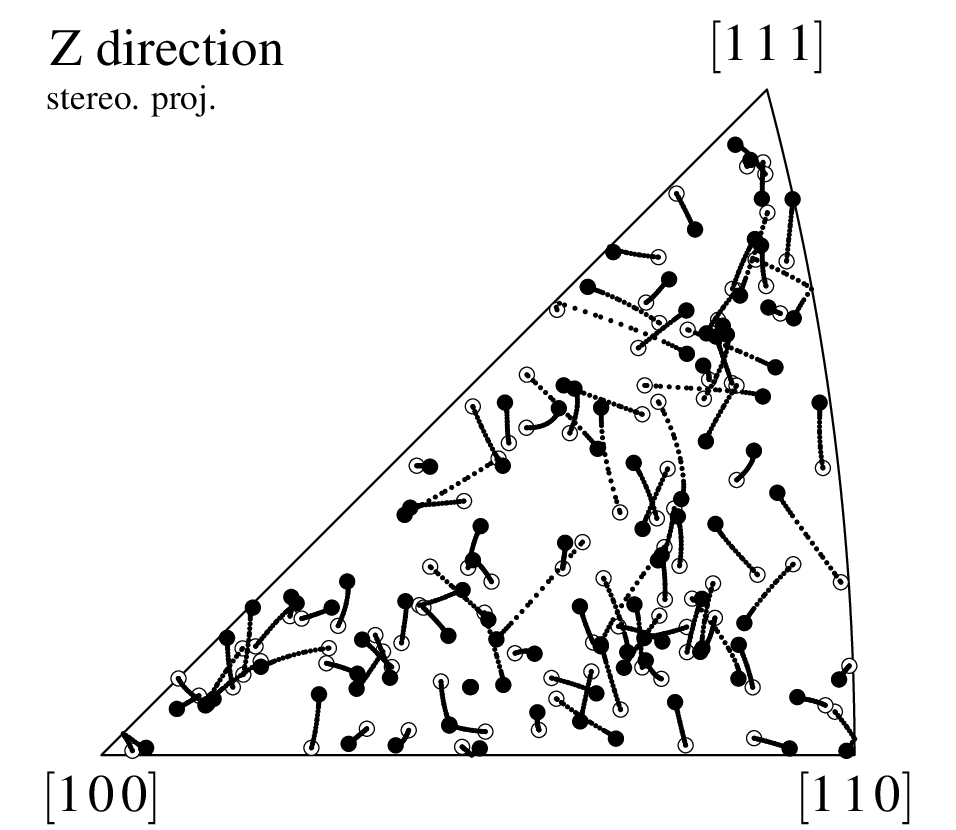
\includegraphics[width=\widF]{figures/testing_fig.png}}
%
\newcommand{\tablee}[1]{ 
\scriptsize{
    \begin{tabular}{|c|c|c|c|c|c|c|c|c|c|c|c|c|}
        \hline
        Simulation &$\hkl(0 1 -1)$ $\hkl[1 1 1]$   &$\hkl(1 0 -1)$ $\hkl[1 1 1]$   &$\hkl(1 -1 0)$ $\hkl[1 1 1]$   &$\hkl(0 1 1)$  $\hkl[1 1 -1]$  &$\hkl(1 0 1)$  $\hkl[1 1 -1]$  &$\hkl(1 -1 0)$ $\hkl[1 1 -1]$  &$\hkl(0 1 1)$  $\hkl[1 -1 1]$  & $\hkl(1 0 -1)$ $\hkl[1 -1 1]$  &$\hkl(1 1 0)$  $\hkl[1 -1 1]$  &$\hkl(0 1 -1)$ $\hkl[1 -1 -1]$ &$\hkl(1 0 1)$  $\hkl[1 -1 -1]$ &$\hkl(1 0 1)$  $\hkl[1 -1 -1]$ \\ \hline \hline
        %\hline
        %&0&1&2&3&4&5&6&7&8&9&10&11\\
         Strength #    & 39.0    & 39.0    & 39.0    & 39.0& 39.0   & 39.0     & 39.0    & 39.     0& 39.0     & 39.0   & 39.0    & 39.0    \\ \hline             
    \end{tabular}}
}
%
\newcommand{\simulation}[3]{
\begin{frame}{Simset number #3}
    \begin{table}[]
        \centering
        \begin{tabular}{|c|ccccc|} 
        \hline
        Domain & 125\% & 150\% & 175\% & 200\% & 400\% &
        \hline
             \polycube&      \cTimesOTF{#1}{#2}& \cTimesOFO{#1}{#2}& \cTimesOSF{#1}{#2}& \cTimesTH{#1}{#2}& \cTimesFH{#1}{#2} \\
             \hline
             \polyelongated& \eTimesOTF{#1}{#2}& \eTimesOFO{#1}{#2}& \eTimesOSF{#1}{#2}& \eTimesTH{#1}{#2}& \eTimesFH{#1}{#2}\\
            \hline
        \end{tabular}
        \label{tab:my_label}
    \end{table}
    \tablee{#3}
\end{frame}

}
% if sim set number <= 25 #1=2, 4 if 25<=simnum<=50 6 if <=75
% #2 = sim setnumber/25 mod 5

\simulation{2}{1}{001-005}
\simulation{1}{1}{005-010}

% Include reference slide here
\begin{frame}{References}
\nocite{*}
\bibliographystyle{unsrt}
\bibliography{bibliography.bib}
\end{frame}

%%%%% End document
\end{document}
